% Streamlines visualization
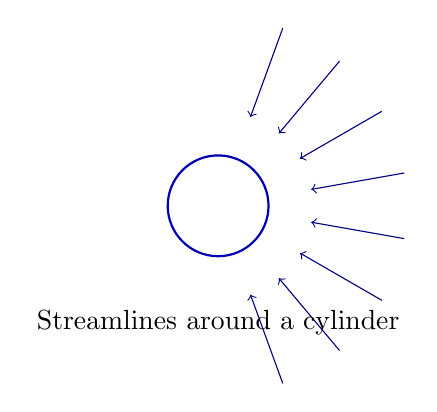
\begin{tikzpicture}[scale=0.8]
  % Flow lines around obstacle
  \draw[blue!70!black, thick] (0,0) circle (0.8);
  \foreach \a in {10,30,50,70,-10,-30,-50,-70} {
    \draw[->, blue!50!black] ({\a}:3) to[out={\a+180}, in={\a}] ({\a}:1.5);
  }
  \node[below] at (0,-1.5) {Streamlines around a cylinder};
\end{tikzpicture}
